%\newcommand{\linhalayout}[2]{{\tiny\textbf{#1}\quad#2\par}}
\newcommand{\linha}[2]{\ifdef{#2}{\linhalayout{#1}{#2}}{}}

\begingroup\tiny
\parindent=0cm
\thispagestyle{empty}

\textbf{Gerência editorial}\quad			 {Ana Mortara}\\
\textbf{Assistência editorial}\quad			 {Paula Dias}\\
\textbf{Assistência administrativa editorial}\quad {Gisele Cerchiaro}\\

\hspace{-5pt}\begin{tabular}{ll}
\textbf{Elaboração de conteúdo} & Abraão Augusto (Língua Portuguesa),	\\
								& Alessandra Domingues Juliano (Língua Portuguesa),	\\
								& Ana Paula Souza Rios (Língua Portuguesa),	\\
								& André Sanchez Astorino (Língua Portuguesa e Língua Inglesa),	\\
								& Clarissa Ayres Mendes (Língua Portuguesa),	\\
								& Eduardo Toniolo Campos (Matemática),	\\
								& Fernanda Dobashi (Língua Portuguesa),	\\
								& Guilherme Salles (Ciências Humanas),	\\
								& Letícia Leme (Ciências Humanas),	\\
								& Lucas Della Santina (Educação Física),	\\
								& Pilar Espí (Arte),	\\
								& Renata Cândido Carvalho (Ciências da Natureza),	\\
								& Thiago Figueiredo (Matemática),	\\
								& Victor Marques (Ciências da Natureza)	\\
\end{tabular}


\textbf{Edição}\quad	 {Carlos Rogério Duarte Barreiros, Fábia Alvim, Felipe Augusto Neves Silva}\\
\textbf{Preparação e revisão}\quad			 {Saíra Editorial}\\
\textbf{Coordenação de arte}\quad			 {Jorge Sallum}\\
\textbf{Editoração eletrônica}\quad			 {Paulo Henrique Pompermaier}\\
\textbf{Pesquisa iconográfica}\quad			 {Margarita Veloso}\\
<<<<<<< HEAD
\textbf{Projeto gráfico e capa}\quad		 {Luísa Marcelino}\\
\textbf{Código}\quad {\ifdef{\RevisionInfo{}}{\RevisionInfo{} (\today, \currenttime)}{001}\medskip}

\noindent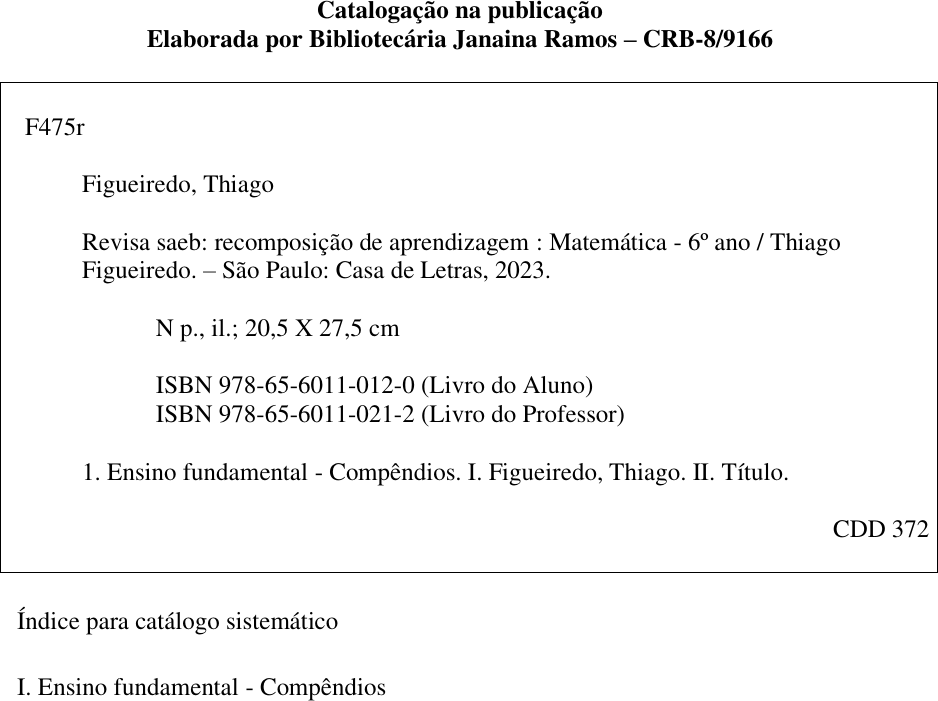
\includegraphics[width=.5\textwidth]{../fichas/6MAT.png}
=======
\textbf{Projeto gráfico e capa}\quad		 {Luísa Marcelino} \\
\textbf{Código}\quad {\ifdef{\RevisionInfo{}}{\RevisionInfo{} (\today, \currenttime)}{001}\medskip}

\noindent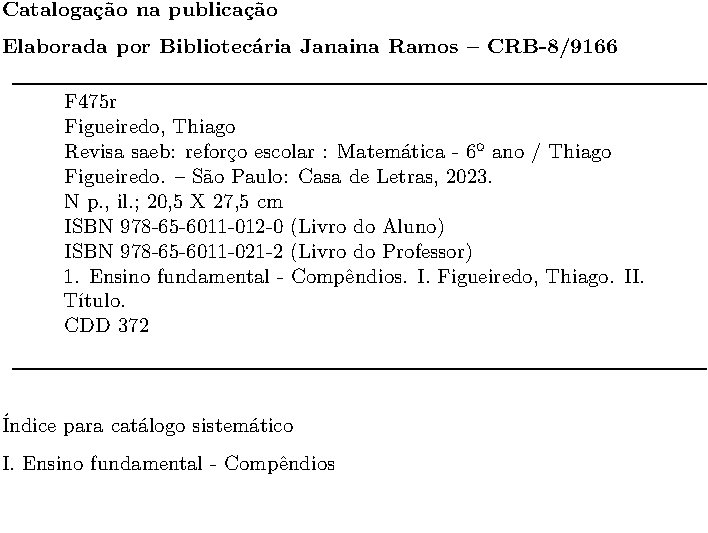
\includegraphics[width=.8\textwidth]{../fichas/6MAT.pdf}
>>>>>>> de81e2747ad296d11187a100c5d83b53b6df0775

\vfill

\textsc{casa de letras e gráfica ltda.}\\
Rua Fradique Coutinho, 1139, andar 2, sala 2\\
CEP 05416--011 -- São Paulo/\textsc{sp}, Brasil\\
Telefone: (11) 3914--7790\\\smallskip
www.casadeletras.com.br\\

\endgroup
\pagebreak
